\documentclass[a4paper,10pt]{article}
\usepackage[utf8]{inputenc}
\usepackage{graphicx}
\usepackage{hyperref}
\usepackage{verbatim}
\usepackage[top=2.54cm,bottom=2.54cm,left=2.54cm,right=2.54cm]{geometry}

%opening
\title{SEng 468 Documentation\\Daytrading Inc.}
\author{Shae Brown, Jarred Hawkins, Brady Schnell}

\begin{document}

\maketitle

\tableofcontents

\section{Architecture}
\subsection{Current System Architecture}
For quickly achieving a one user workload in the day trading application, a 
minimal system architecture was used. The graph below demonstrates the 
architecture that was used to support a one user workload.

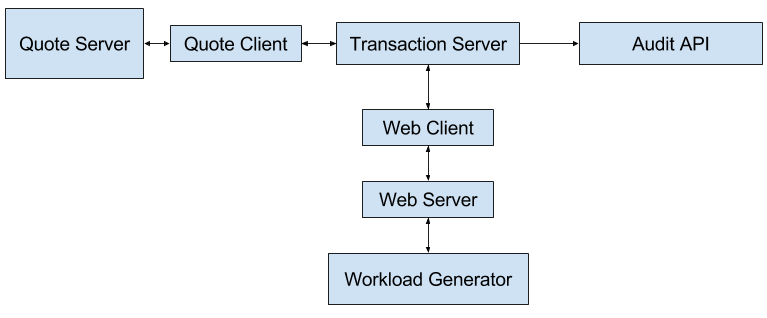
\includegraphics[width=0.9 \linewidth]{./arch.png}

The workload generator simulates a users interaction with the system by taking a 
list of commands, and then sending HTTP requests to the appropriate web server 
endpoints. The web server matches the HTTP request to the particular endpoint, 
and then the Web client forwards the request to the respective transaction 
server endpoint.

The transaction server is where the bulk of the processing is currently done. 
All user actions are executed within the transaction server. The transaction 
server currently tracks the current user's id, account funds, and stocks. 
Additionally, the transaction server sends a message to the quote client which 
will query the quote server with the specified action. The quote client then 
returns the result of the query back to the transaction server for any further 
processing.

Upon receiving a command, the transaction server makes a call to the Audit API 
to log the requested command. Further calls to the audit API may be made 
depending on if the user's command was executed successfully, or if an error 
occurred.

Once a command has been completed, the transaction server will return a message 
to the Web Client to indicate whether the command was a success or a failure. 
The web client then processes the response from the transaction server, and 
creates a corresponding HTTP status code message. The web client then passes the 
HTTP status code back to the web server which then sends the HTTP response back 
to the Workload generator. 

Finally, the workload generator parses the response and determines if the 
command was successful or not. After all commands have been executed, the 
workload generator gives a report of the total number of successful and 
unsuccessful commands.

\subsection{Project Plan}

\subsubsection{Weekly Deadlines}
\begin{itemize}
\item First log book entries are due Jan 19th by 23:59:59
\item Log book entries (must be completed individually by each group member and 
signed by the entire group - 1\% deducted for each missing/late log book entry 
to a maximum of 5\% of the project mark)
\end{itemize}


\begin{itemize}
 \item Jan 26th: Verified execution of 1 user workload file
 \item Jan 29th: Documentation
  \begin{itemize}
	\item Project Plan
	\item Initial Requirements
	\item Architecture
  \end{itemize}
 \item Feb 9th	Verified execution of 10 user workload file
\item Feb 16th Verified execution of 45 user workload file\\
Requires:\\
- prep multiple instances of components (either auto scale or deploy enough in 
advance)

\item Feb 23d	Verified execution of 100 user workload file\\
Requires:
- deal with scaling issues as they persist

\item Mar 9th	Verified execution of 1000 user workload file\\
Requires:
- deal with scaling issues as they persist
- optimise performance

Note: just under a month here, then final deadlines hit
This means we have lots of time to do these optimisations, along with report 
writing and presentations. 

- polish web interface
- report writing
- presentation prep

\item April 4th
Group project presentations during regular class time
Presentation schedule will be announced in class, end of March
Students must attend all presentation days

\item April 4th Demonstration of web interface (must be booked with your TA by 
March 24th)

\item April 8th Verified execution of final 2018 workload file by 16:59:59.

\item April 11th
- Submission of final project reports, printed and in PDF format, by 16:59:59
- Submission of all project source code via email to TA
\end{itemize}

\subsubsection{Grading}
\begin{itemize}
 \item 5\%	Transaction and cost performance relative to the other groups
 \item 5\%	Overall Architecture and Documentation, including Project Plan
 \item 5\%	Security Design, Analysis and Documentation
 \item 5\%	Test Plan Design, Analysis, and Documentation
 \item 5\%	Fault Tolerance Design, Analysis, and Documentation
 \item 5\%	Performance Analysis, Testing, and Documentation
 \item 5\%	Capacity Planning Analysis, Measurement, and Documentation
 \item 5\%	Project Presentation
 \item -1\%	Each missing (or late) log book entry  (assessed individually)
 \item -1\%	Each missing (or late) milestone deliverable (assessed on a group 
basis)
\end{itemize}

\subsection{Requirements}
\subsubsection{Ports}
Quoteserver: 4450\\
Inter-Lab comms: 44455 - 44459

\subsubsection{User Commands}

Document describing all available commands is available at 
\href{http://www.ece.uvic.ca/~seng462/ProjectWebSite/Commands.html}{the course 
website}. All of the above commands must be supported from the client console. 
The ability to dump a log of all transactions must be supported from a 
supervisory client (implement as part of the group project web site)

\subsubsection{Software rules}
\begin{itemize}
\item DayTrading Inc. requires that the project be build using Docker 
Container technologies. All other software choices are open to each group to 
make, along with the responsibility to install, maintain, come up to speed on, 
etc. the full technology stack used. All groups must use a full proper code 
repository for their project.
\item Caching strategies may be applied to reduce the quote server access time, 
but all business rules and specification must still be met.
\item Inputs and outputs of the Stock Quote Server are ASCII strings of the 
following format:
\\Server Command Format: “StockSymbol, USERNAME”
\\Server Quote Return Format: “Quote, StockSymbol, USERNAME, CryptoKey”
\end{itemize}


\subsubsection{Business rules}
\textit{\\Note: All business rules are peculiarities derived from the specs
document.}

\begin{itemize}
\item Provide acceptable performance, reliability, fault tolerance
\item Minimum transaction processing times.
\item Full support for required features.
\item Reliability and maintainability of the system.
\item High availability and fault recoverability (i.e. proper use of fault 
tolerance)
\item Full persistence for all transaction and accounting operations.
\item Minimal costs (development, hardware, maintenance, etc.)
\item Clean design that is easily understandable and maintainable.
\item Appropriate security
\item A clean web-client interface.
\item Fully supported and complete audit trail
\item Full documentation of architecture including complete analysis of design 
choices.
\item Full documentation of test plans, testing results, and test analyses.
\item Full documentation of work effort required to build prototype, including 
weekly individual log book entries signed by each member of the design team.
\item Complete capacity planning and transaction time documentation, including 
experimental results and extrapolations. 
\item Full security analysis.
\item Full project planning and execution documentation for prototype 
development effort.
\item Full analysis of system capacity and capacity planning documentation

\item All claims within the project documentation must be supported through 
appropriate experimental testing and analysis
\item All documents must be clear, concise, and correct with respect to English
usage and grammar.
\item Documentation that is not comprehensible, overly verbose, rambling, etc. 
willbe viewed by DayTrading Inc. as indicative of the design team’s general 
level of care and attention,and therefore will reflect negatively on the 
team’s overall evaluation. 

\item Each client logs in through a web browser and then performs a number of 
stock trading and account management activities.
\item In addition to the client activities, DayTrading requires full auditing 
capabilities; hence, complete transaction logs must be able to be produced on 
demand that detail of all client activities in thesystem (including timestamps 
of all transactions), a record of each individual transaction, each 
transaction’s processing time information, and all account state changes within 
the system. 
\item This log must be dumped from the system as an ASCII text file when it 
receives the DUMPLOG command.
 
\end{itemize}

\section{Component Documentation}
\subsection{Web Server}
\subsection{Audit Server}
\paragraph{Description}

The audit server is an HTTP web server. For each endpoint, pass the information 
as URI queries. For example, to post a new userCommand event, the request URI 
would be as follows:

\begin{verbatim}
localhost:8080/userCommand?server=TRANS&funds=22.33&transactionNum=11&command=BU 
Y\end{verbatim}

TODO:
\begin{itemize}
 \item Input validiation and error checking
 \item Multithreading requests to write to the log object
 \item Set up and document proper return values
\end{itemize}

\paragraph{Endpoints}

For all supported params, being surrounded with brackets indicates optional.

\begin{itemize}
 \item \textbf{/userCommand}
\\Supported Params:
    server
    transactionNum
    command
    (username)
    (stockSymbol)
    (filename)
    (funds)

 \item \textbf{/quoteServer}
  \\Supported Params:
	 server
	 transactionNum
	 price
	 stockSymbol
	 username
	 quoteServerTime
	 cryptoKey

 \item \textbf{/accountTransaction}
  \\Supported Params:
	 transactionNum
	 action
	 (username)
	 (funds)

 \item \textbf{/systemEvent}
  \\Supported Params:
	 transactionNum
	 command
	 (username)
	 (stockSymbol)
	 (filename)
	 (funds)

 \item \textbf{/errorEvent}
  \\Supported Params:
	 server
	 transactionNum
	 command
	 (username)
	 (stockSymbol)
	 (filename)
	 (funds)
	 (errormessage)

 \item \textbf{/dumpLog}
  \\Supported Params:
	 filename
	 (username)
\end{itemize}

Return Values:
\\Right now the commands just echo the parsed xml.

\subsection{Transaction Server}
The transaction server still handles the core of the logic.

\subsection{Database}
For a database, we chose to use Redis for its scalaiblity, fault tolerance and 
low overhead. In addition, in an iterative course such as this, we value being 
able to change the schema on the fly. Since Redis is a key/value store we kept 
the schema light. The documentation has key in the header, with a description of 
the params in the body. Our redis instance is fully Docker containerized and 
runs well with the default settings.

\paragraph{Endpoints}

Redis uses TCP by default. There are also many clients provided.

\begin{itemize}
\item \textbf{USERID:Balance}
\\Contains the balance of the user ID. Stored as a floating point number for 
now, however Redis does offer some accuracy guarantees.
\\Functions:
   AddFunds
   GetFunds
   RemoveFunds

\item \textbf{USERID:Stocks}
\\Redis hash of the stocks a user owns. Stocks are stored as integers.
\\Functions:
  AddStock
  GetStock
  RemoveFunds

\item \textbf{USERID:SellOrders}
\\Keeps tracks of user's uncomitted sell orders.
\\Functions:
  PushSell
  PopSell

\item \textbf{USERID:BuyOrders}
\\Keeps tracks of user's uncomitted buy orders.
\\Functions:
  PushBuy
  PopBuy

\item \textbf{USERID:SellTriggers}
\\Keeps tracks of user's running triggers.
\\Functions:
  AddSellTrigger
  RemoveSellTrigger
  GetSellTrigger
 
\item \textbf{USERID:BuyTriggers}
\\Keeps tracks of user's running triggers.
\\Functions:
  AddBuyTrigger
  RemoveBuyTrigger
  GetBuyTrigger
  
\item \textbf{USERID:BalanceReserve}
Keeps tracks of user's reserve account balance. This holds funds offset for 
triggers
\textit{Not implemented yet}

\item \textbf{USERID:StocksReserve}
Keeps tracks of user's waiting sell triggers balance.
\textit{Not implemented yet}

\item \textbf{USERID:History}
Keeps tracks of all user's account transactions.

\textit{Not implemented yet}

\item \textbf{Other functions}
  GetUserInfo: Returns as user's account information
\end{itemize}
Running
  Build the docker container.  Expose the proper ports when running (-p 
exposed:6397).  Good to go!

\end{document}
